% Plot the various performance indicators to illustrate the team choice and various result in data preprocessing & mining
\section{Data Visualization}\label{data_visualisation}

This section encompasses the graphical representation of data features and model architectures for enhanced comprehension.

\begin{description}[style=nextline]
    \item[Feature Visualization:] Visual depiction of both given and derived features for enhanced understanding.
    \item[Convolution Neural Network:] Visual representation of CNN model architecture to facilitate interpretation.
    \item[Multilayer Perceptron:] Visual depiction of MLP model architecture for improved insight into its workings.
\end{description}

%%%%%%%%%%%%%%%%%%%%%%%%%%%%%%%%%%%%%%%%%%%%%%%%%
% Feature Visualisation 
%%%%%%%%%%%%%%%%%%%%%%%%%%%%%%%%%%%%%%%%%%%%%%%%%
\subsection{Feature Visualization}\label{feature_visualization}

\subsubsection{Frequency Graph of LOS and NLOS}\label{frequency_graph}

\begin{figure}[H] 
	\centering
	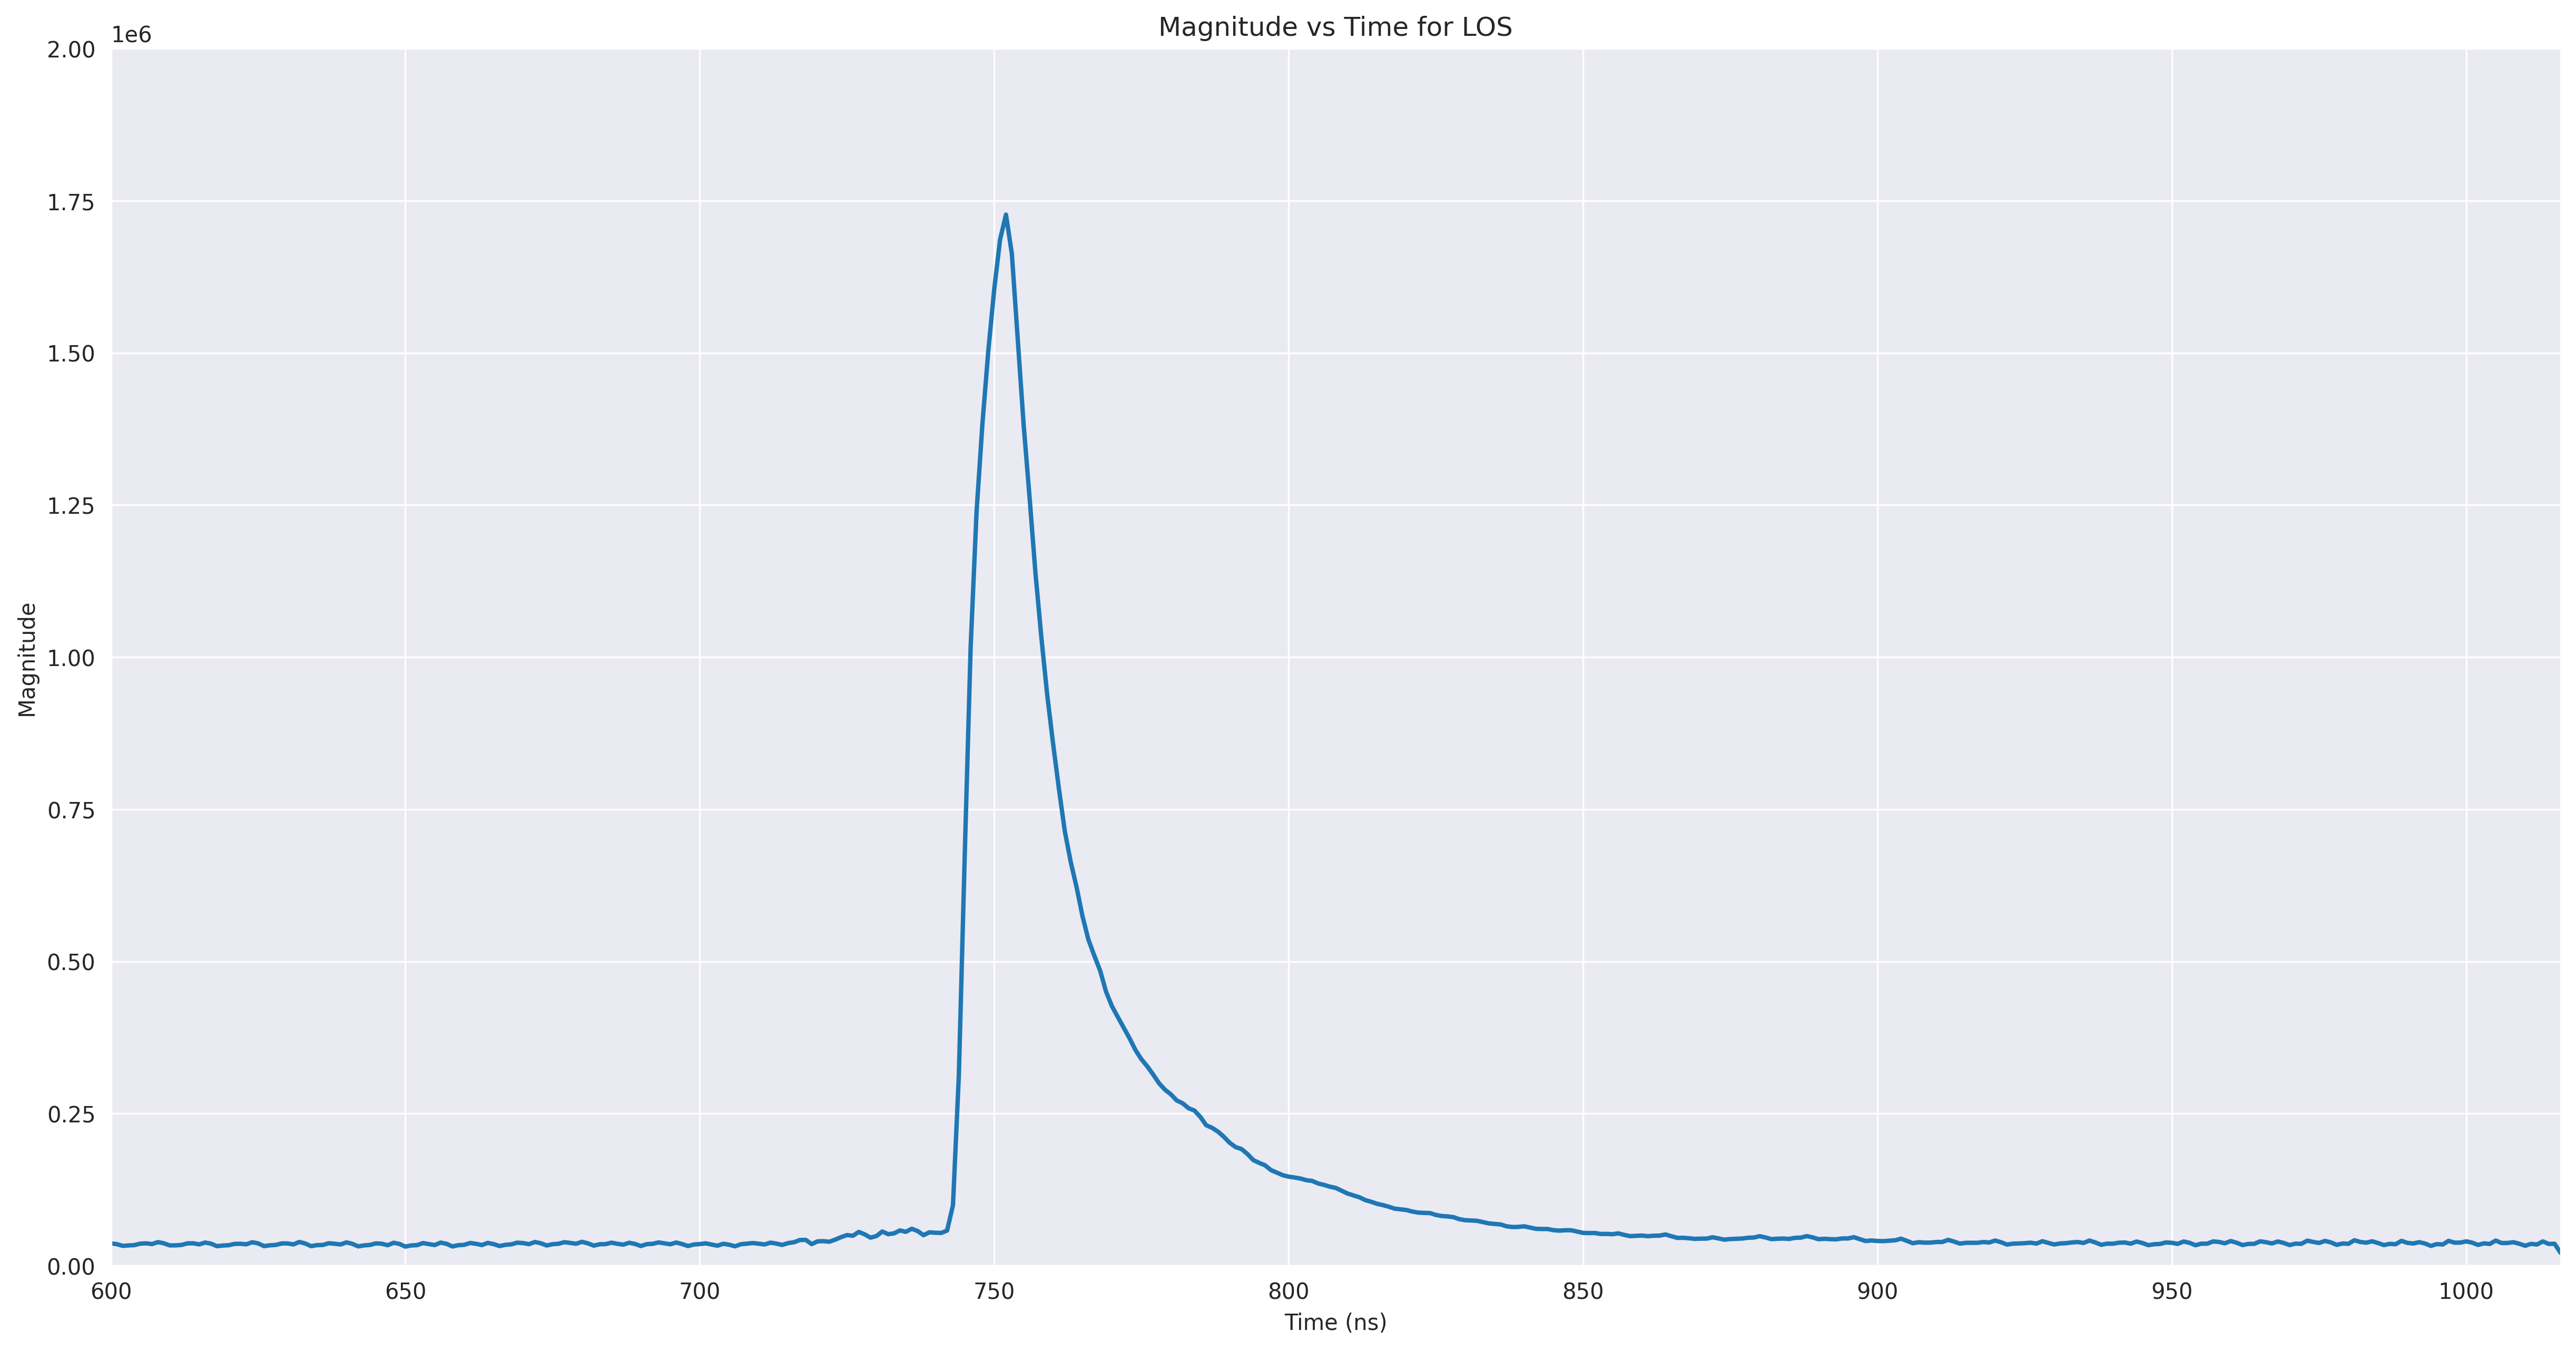
\includegraphics[width=1\textwidth]{preprocessing/LOS_Frequency_Graph.png}
	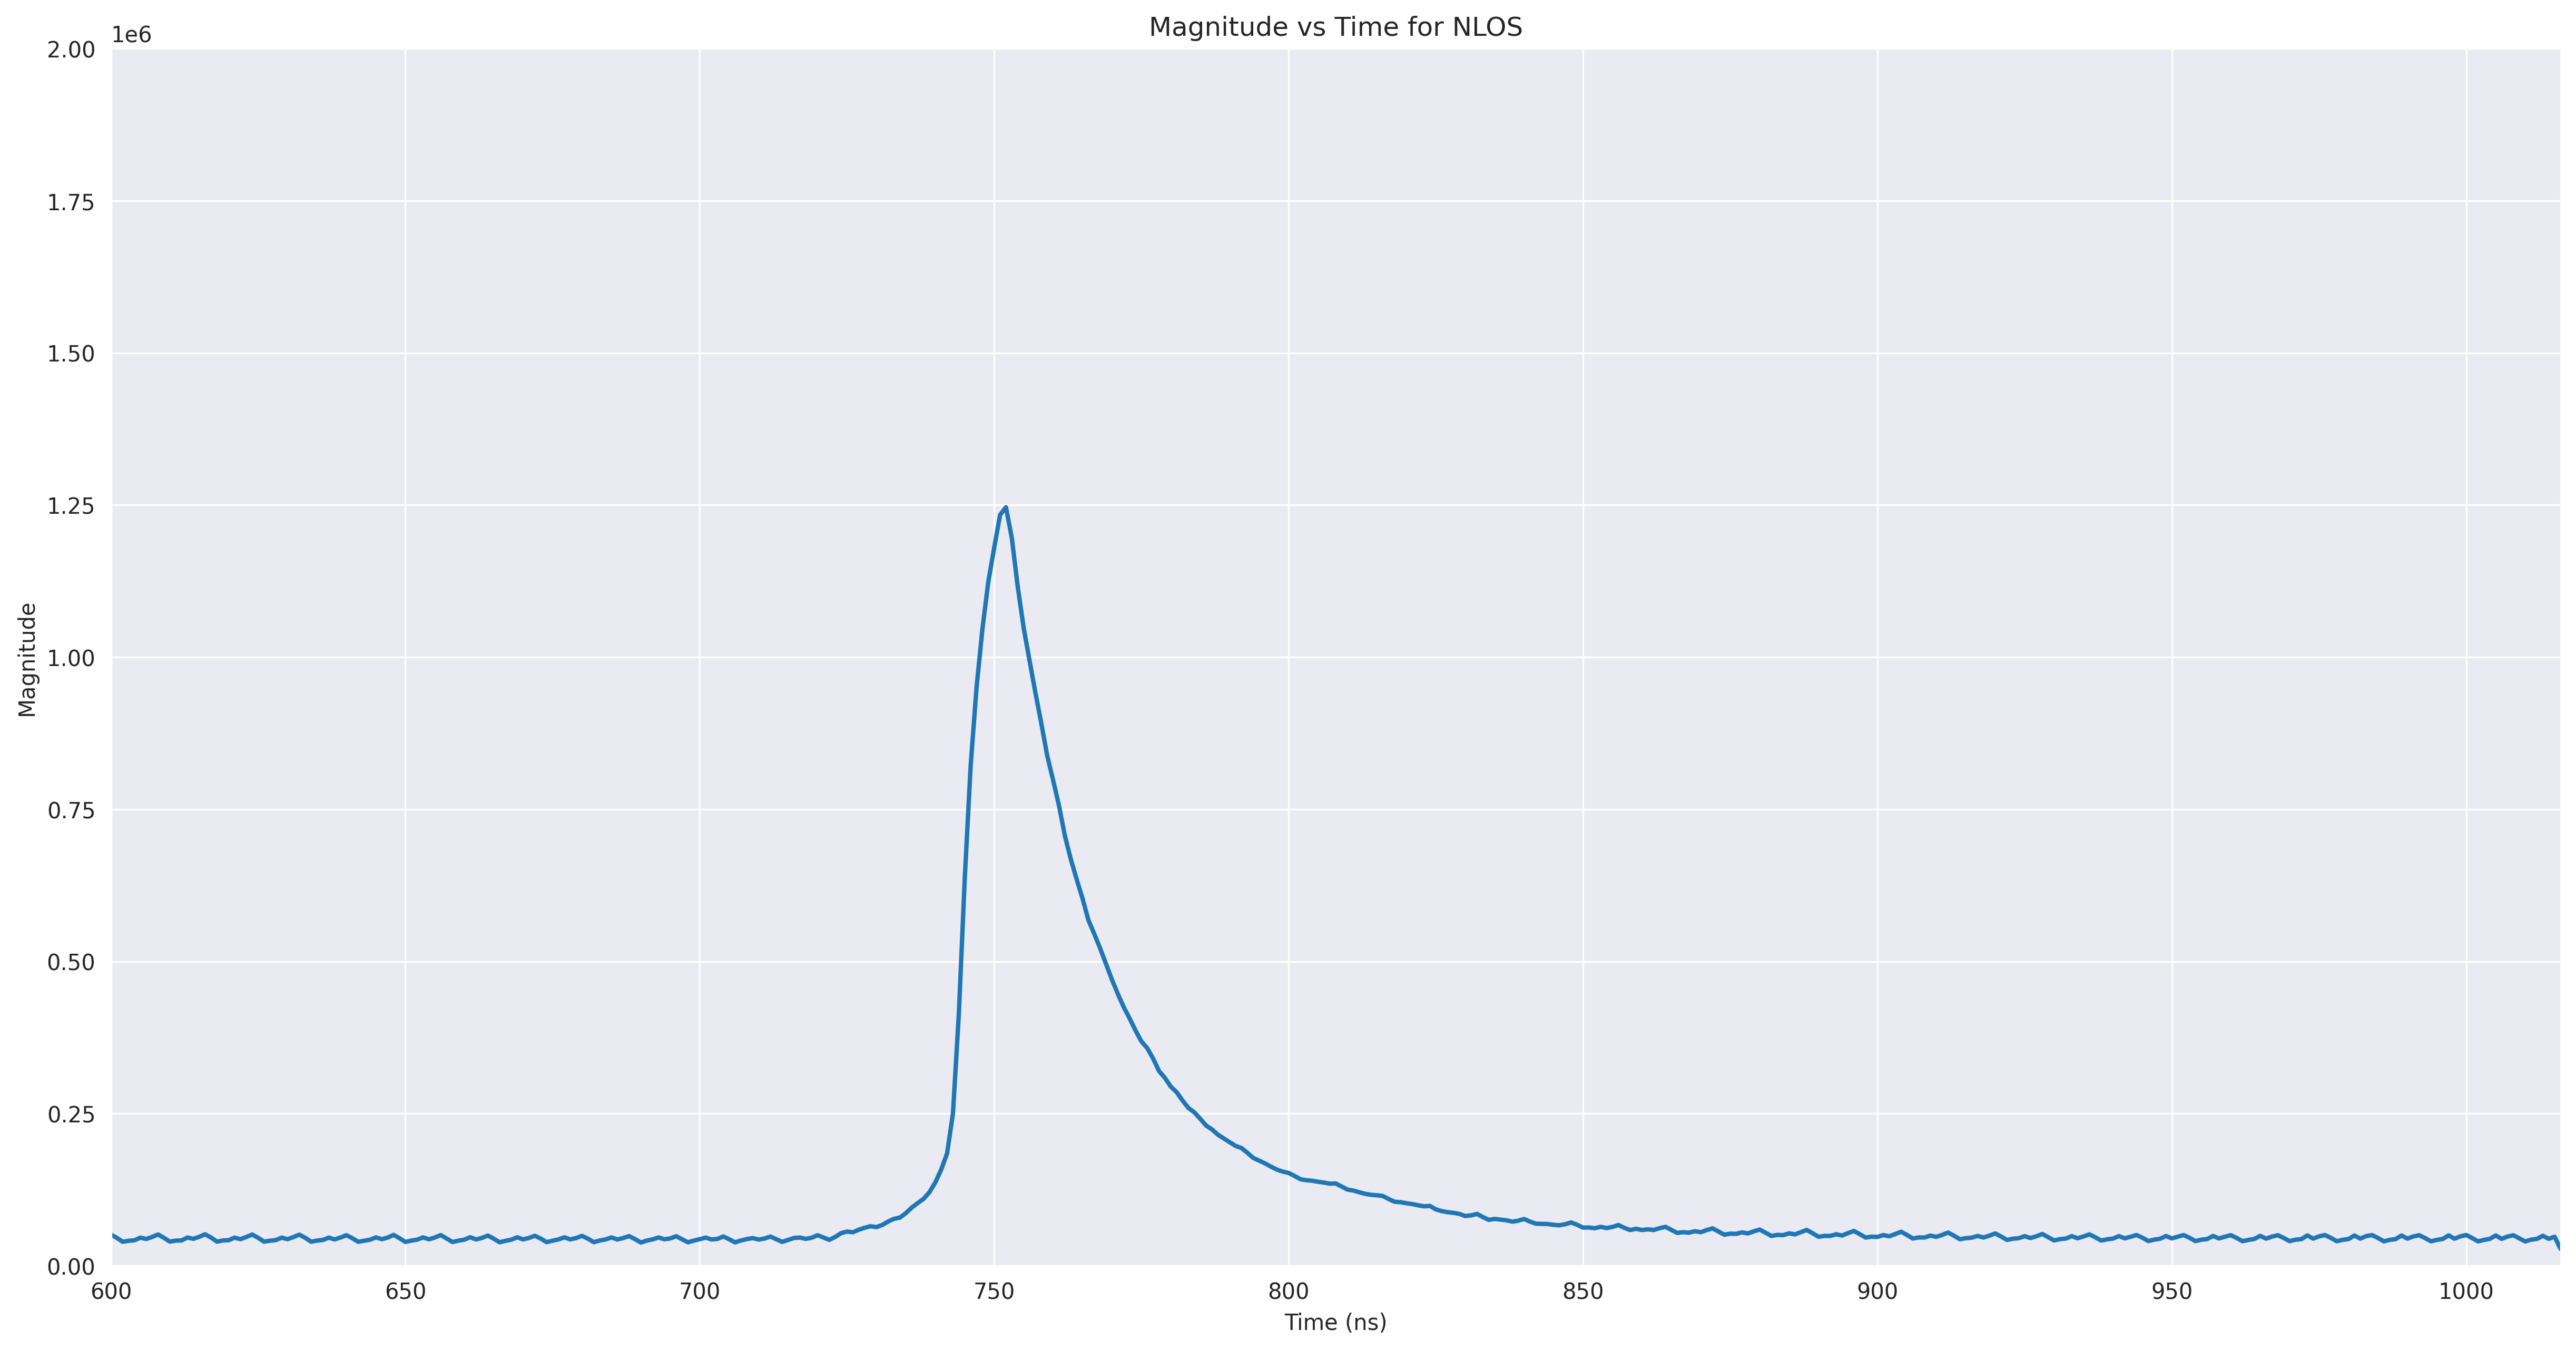
\includegraphics[width=1\textwidth]{preprocessing/NLOS_Frequency_Graph.png}
	\caption{Frequency Graph of LOS and NLOS}\label{fig:frequency_graph}
\end{figure}

\subsubsection{Frequency Graph of Wavelet Transformed LOS and NLOS}\label{frequency_graph_wavelet}

\begin{figure}[H] 
  \centering
  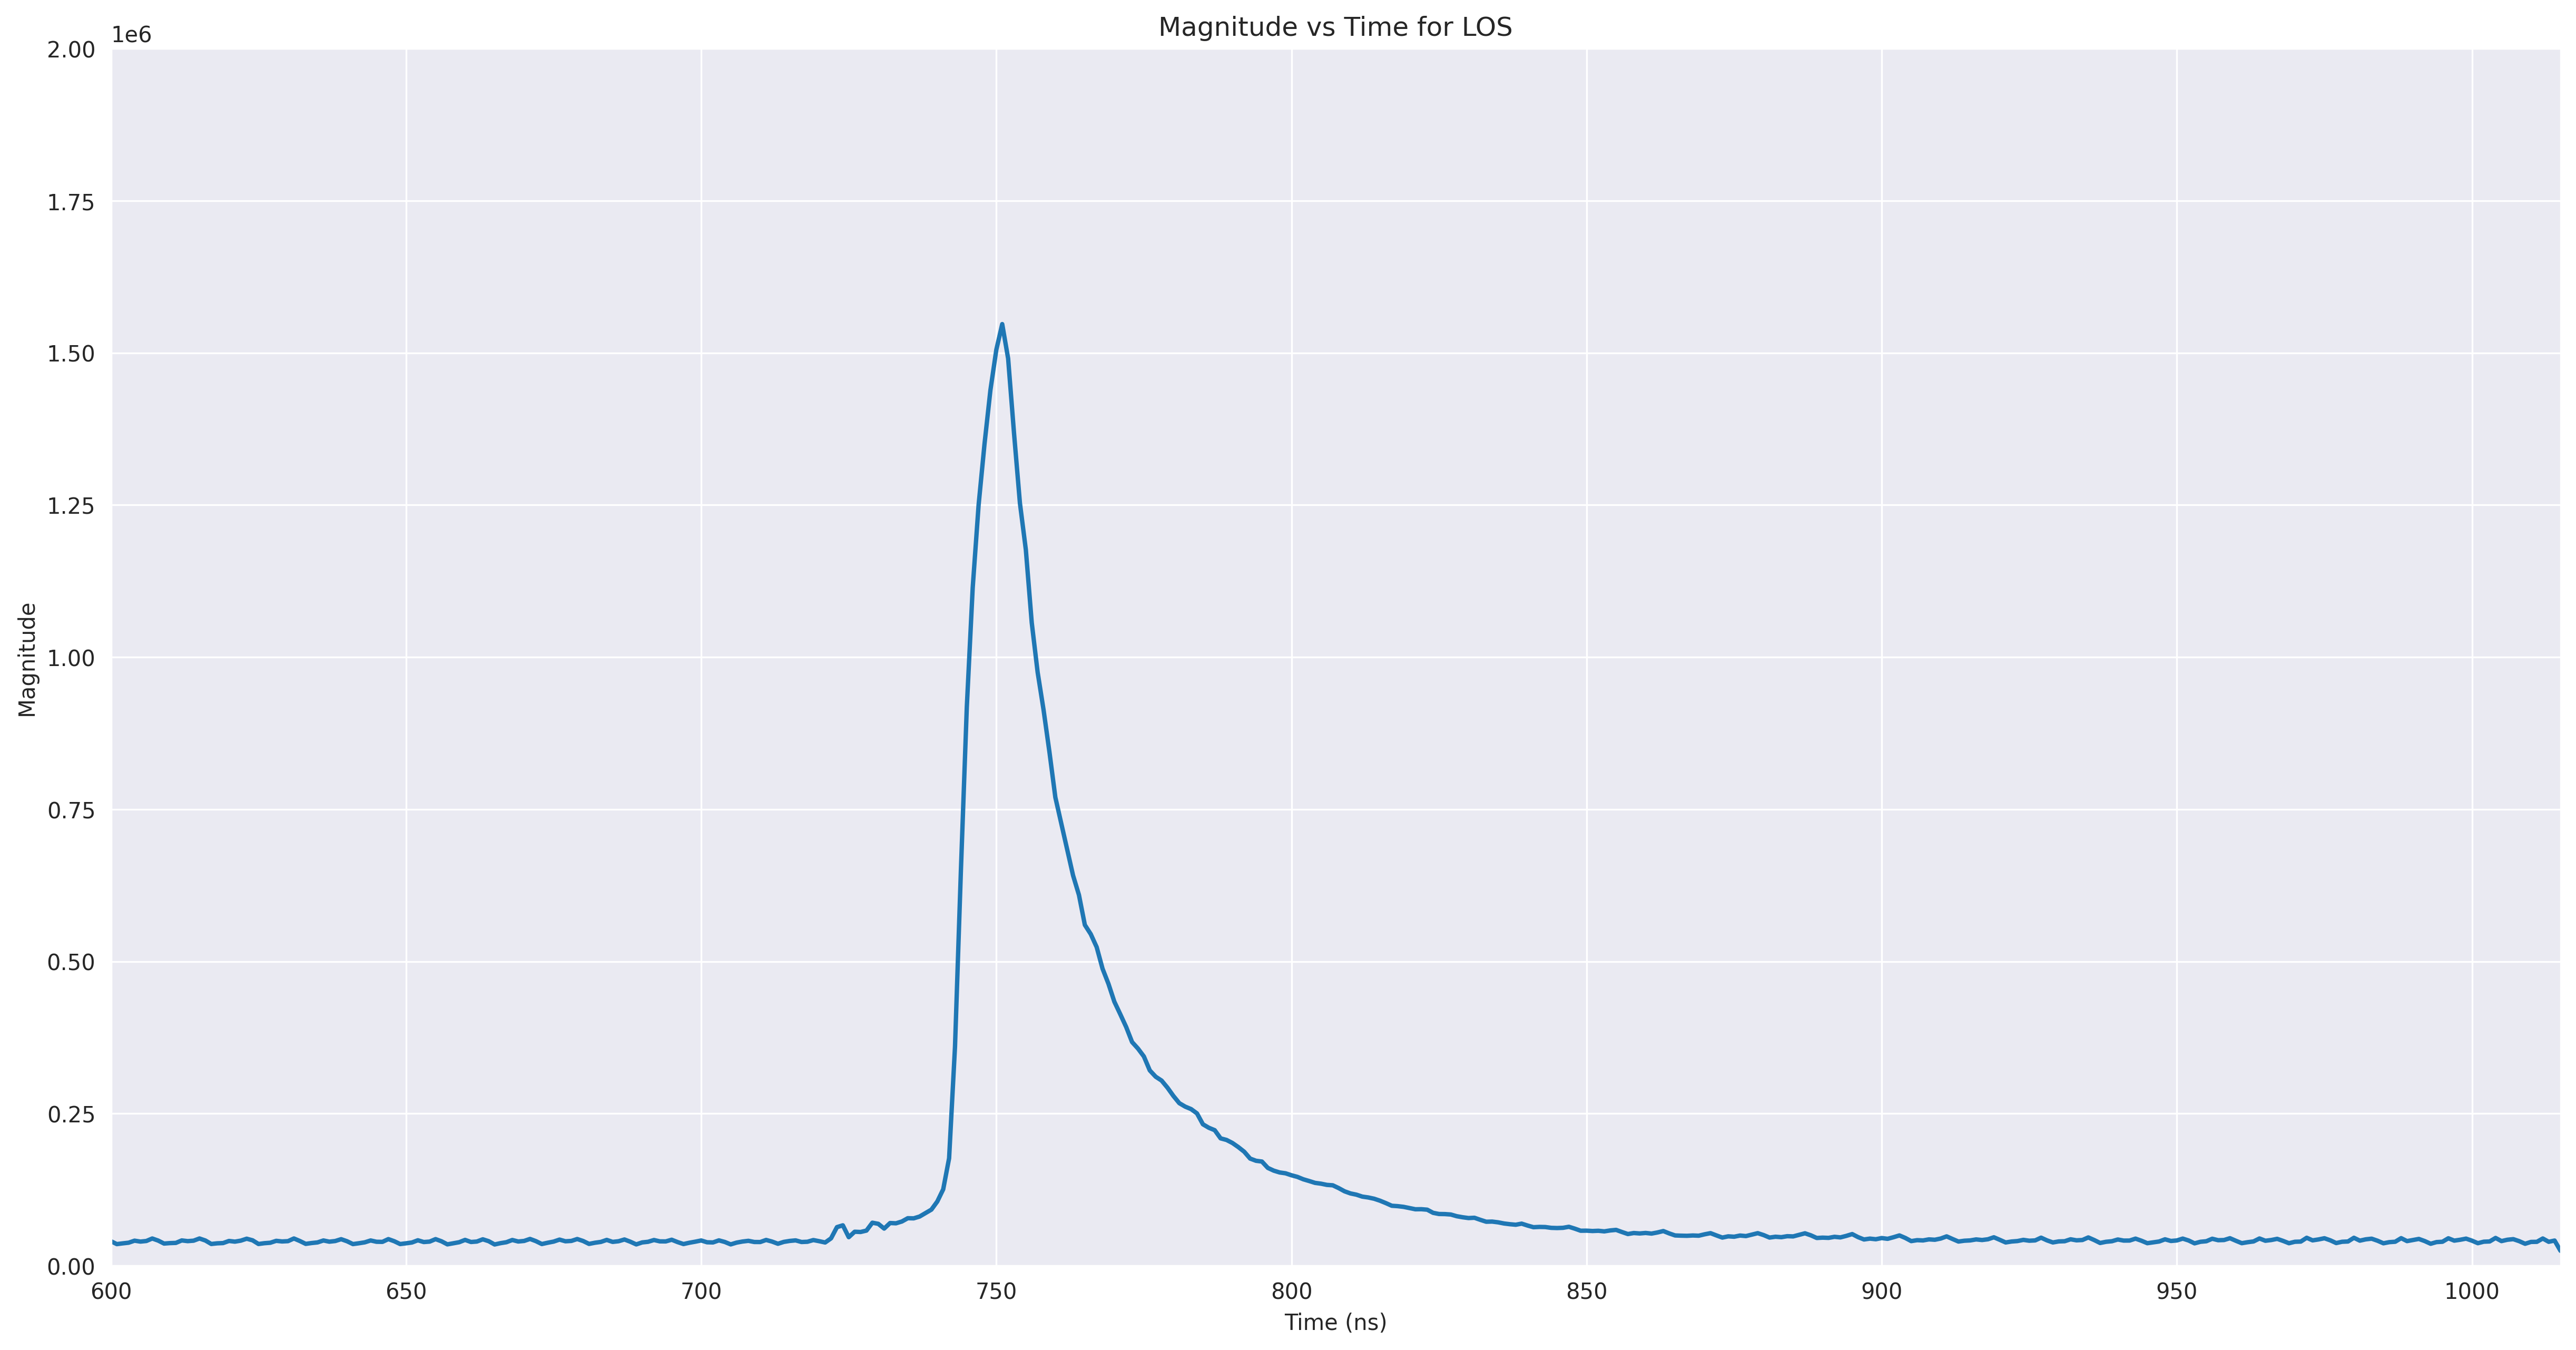
\includegraphics[width=1\textwidth]{preprocessing/Wavelet_Denoised_LOS_Frequency_Graph.png}
  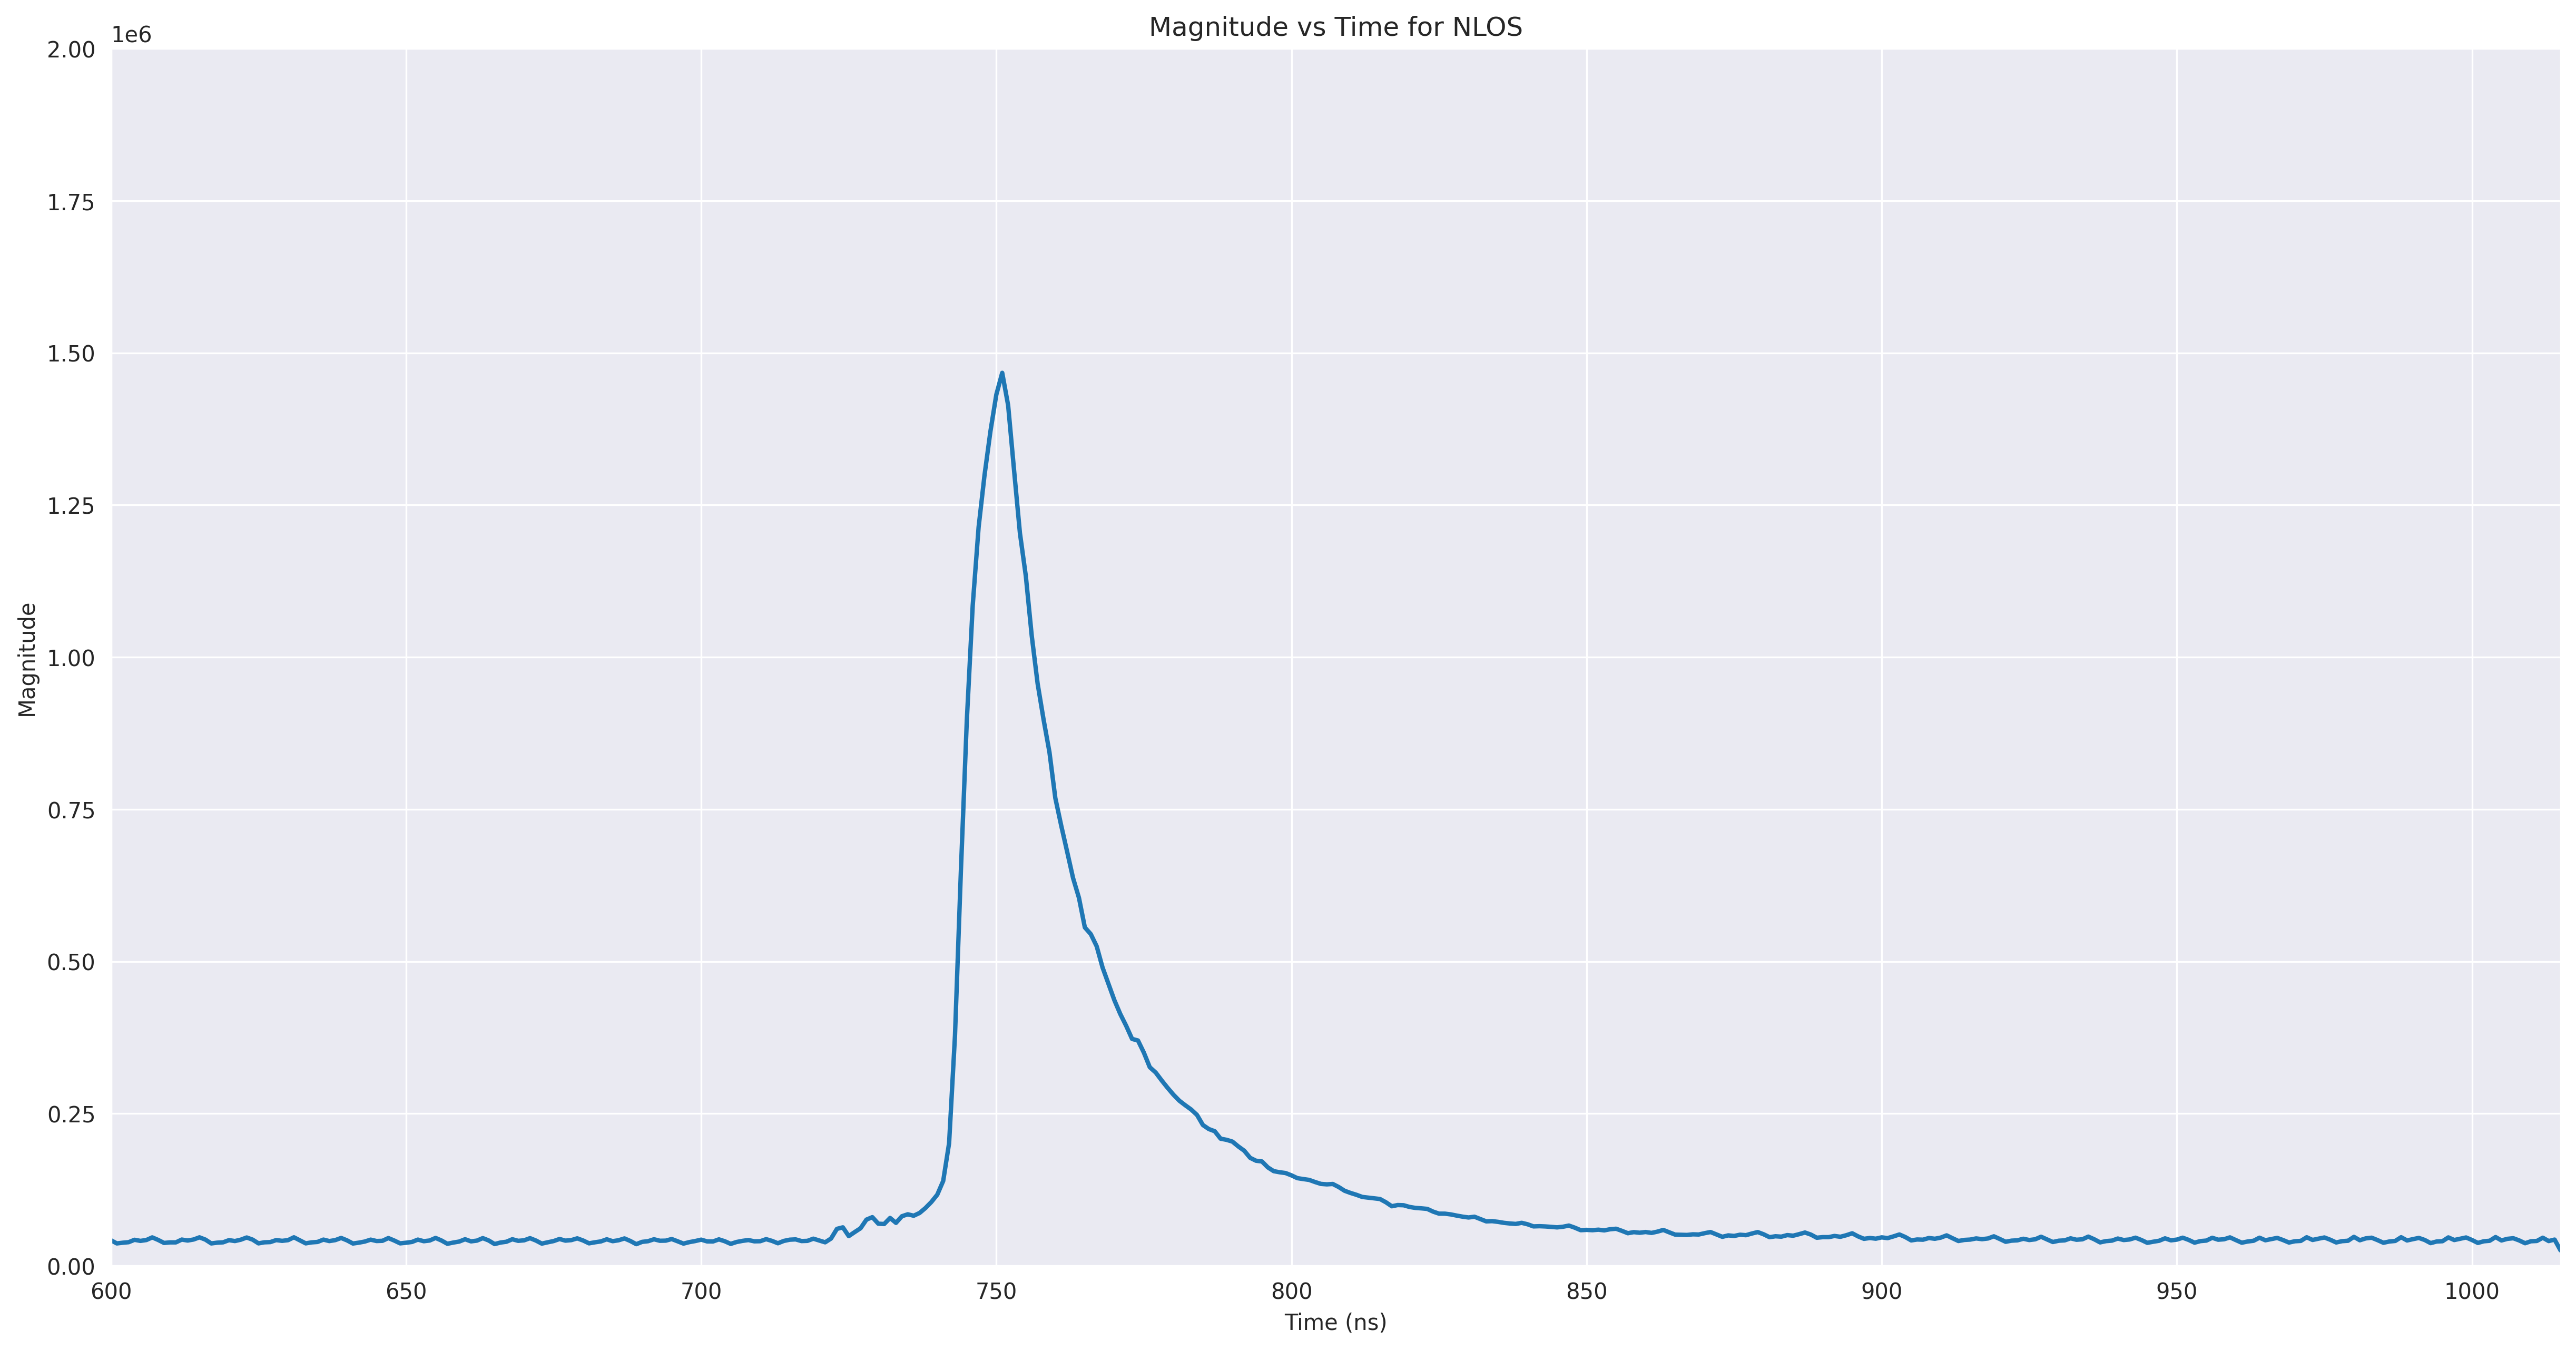
\includegraphics[width=1\textwidth]{preprocessing/Wavelet_Denoised_NLOS_Frequency_Graph.png}
  \caption{Frequency Graph of Wavelet Transformed LOS and NLOS}\label{fig:frequency_graph_wavelet}
\end{figure}

\subsubsection{Frequency Graph of Lucy-Richardson Transformation LOS and NLOS}\label{frequency_graph_lr}

\begin{figure}[H] 
  \centering
  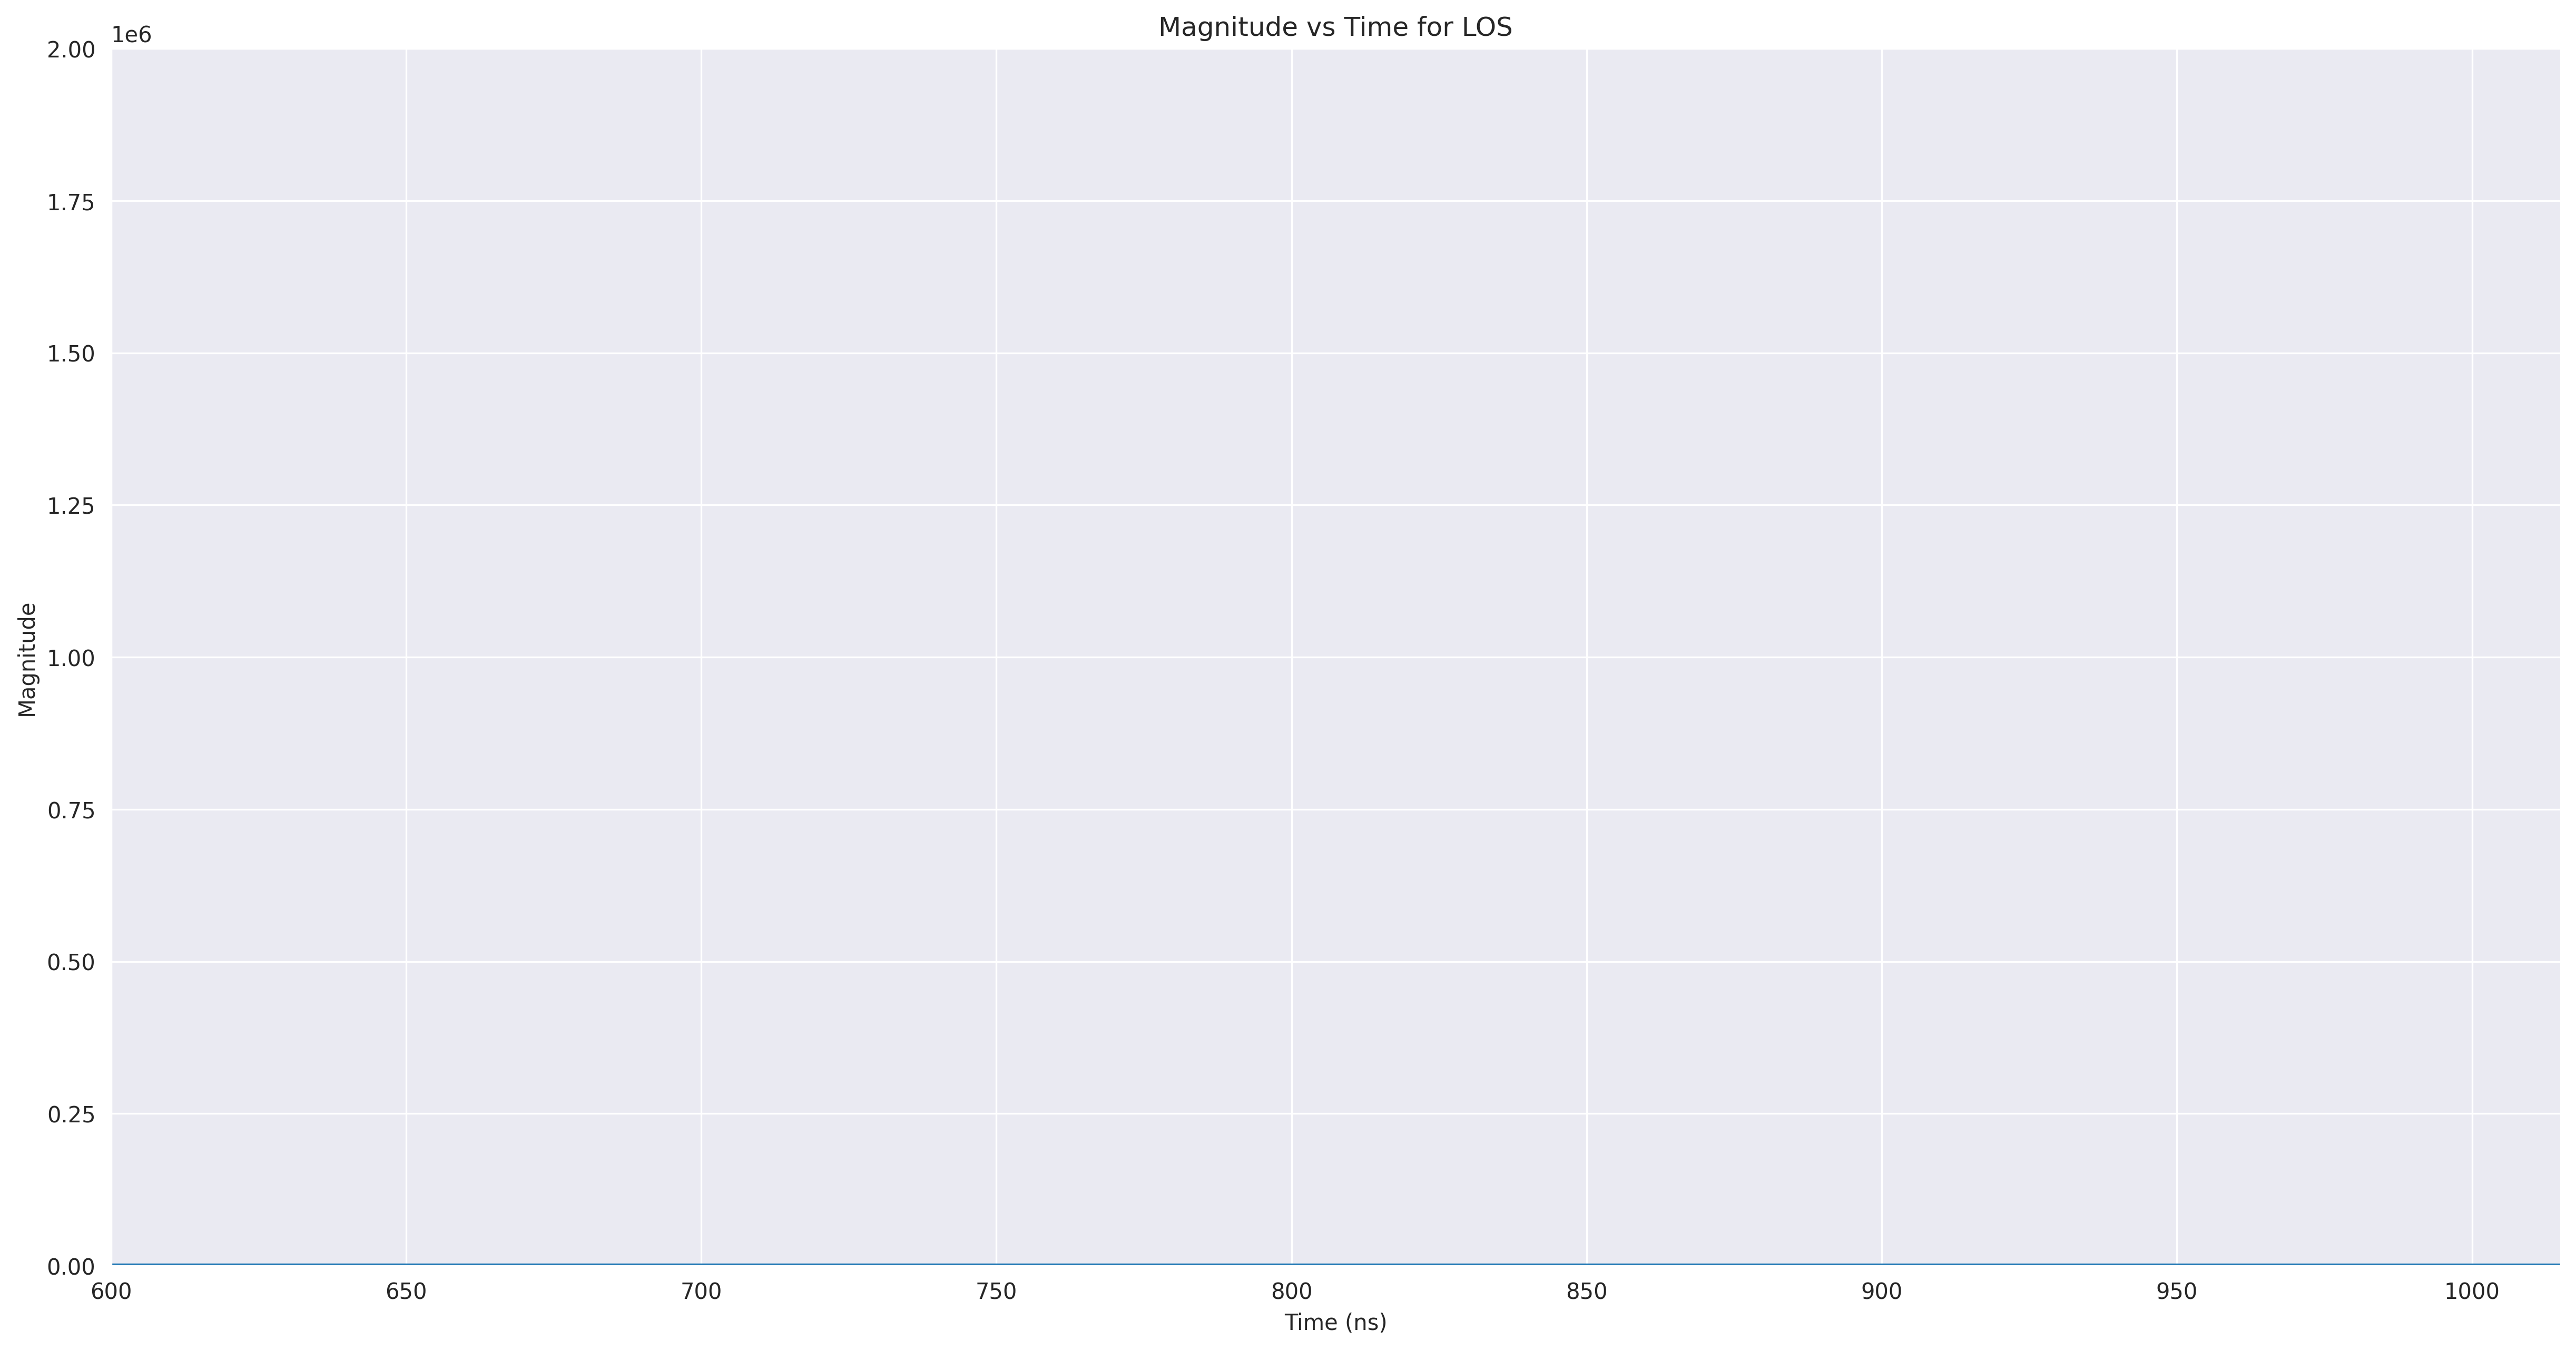
\includegraphics[width=1\textwidth]{preprocessing/lr_denoise_LOS.png}
  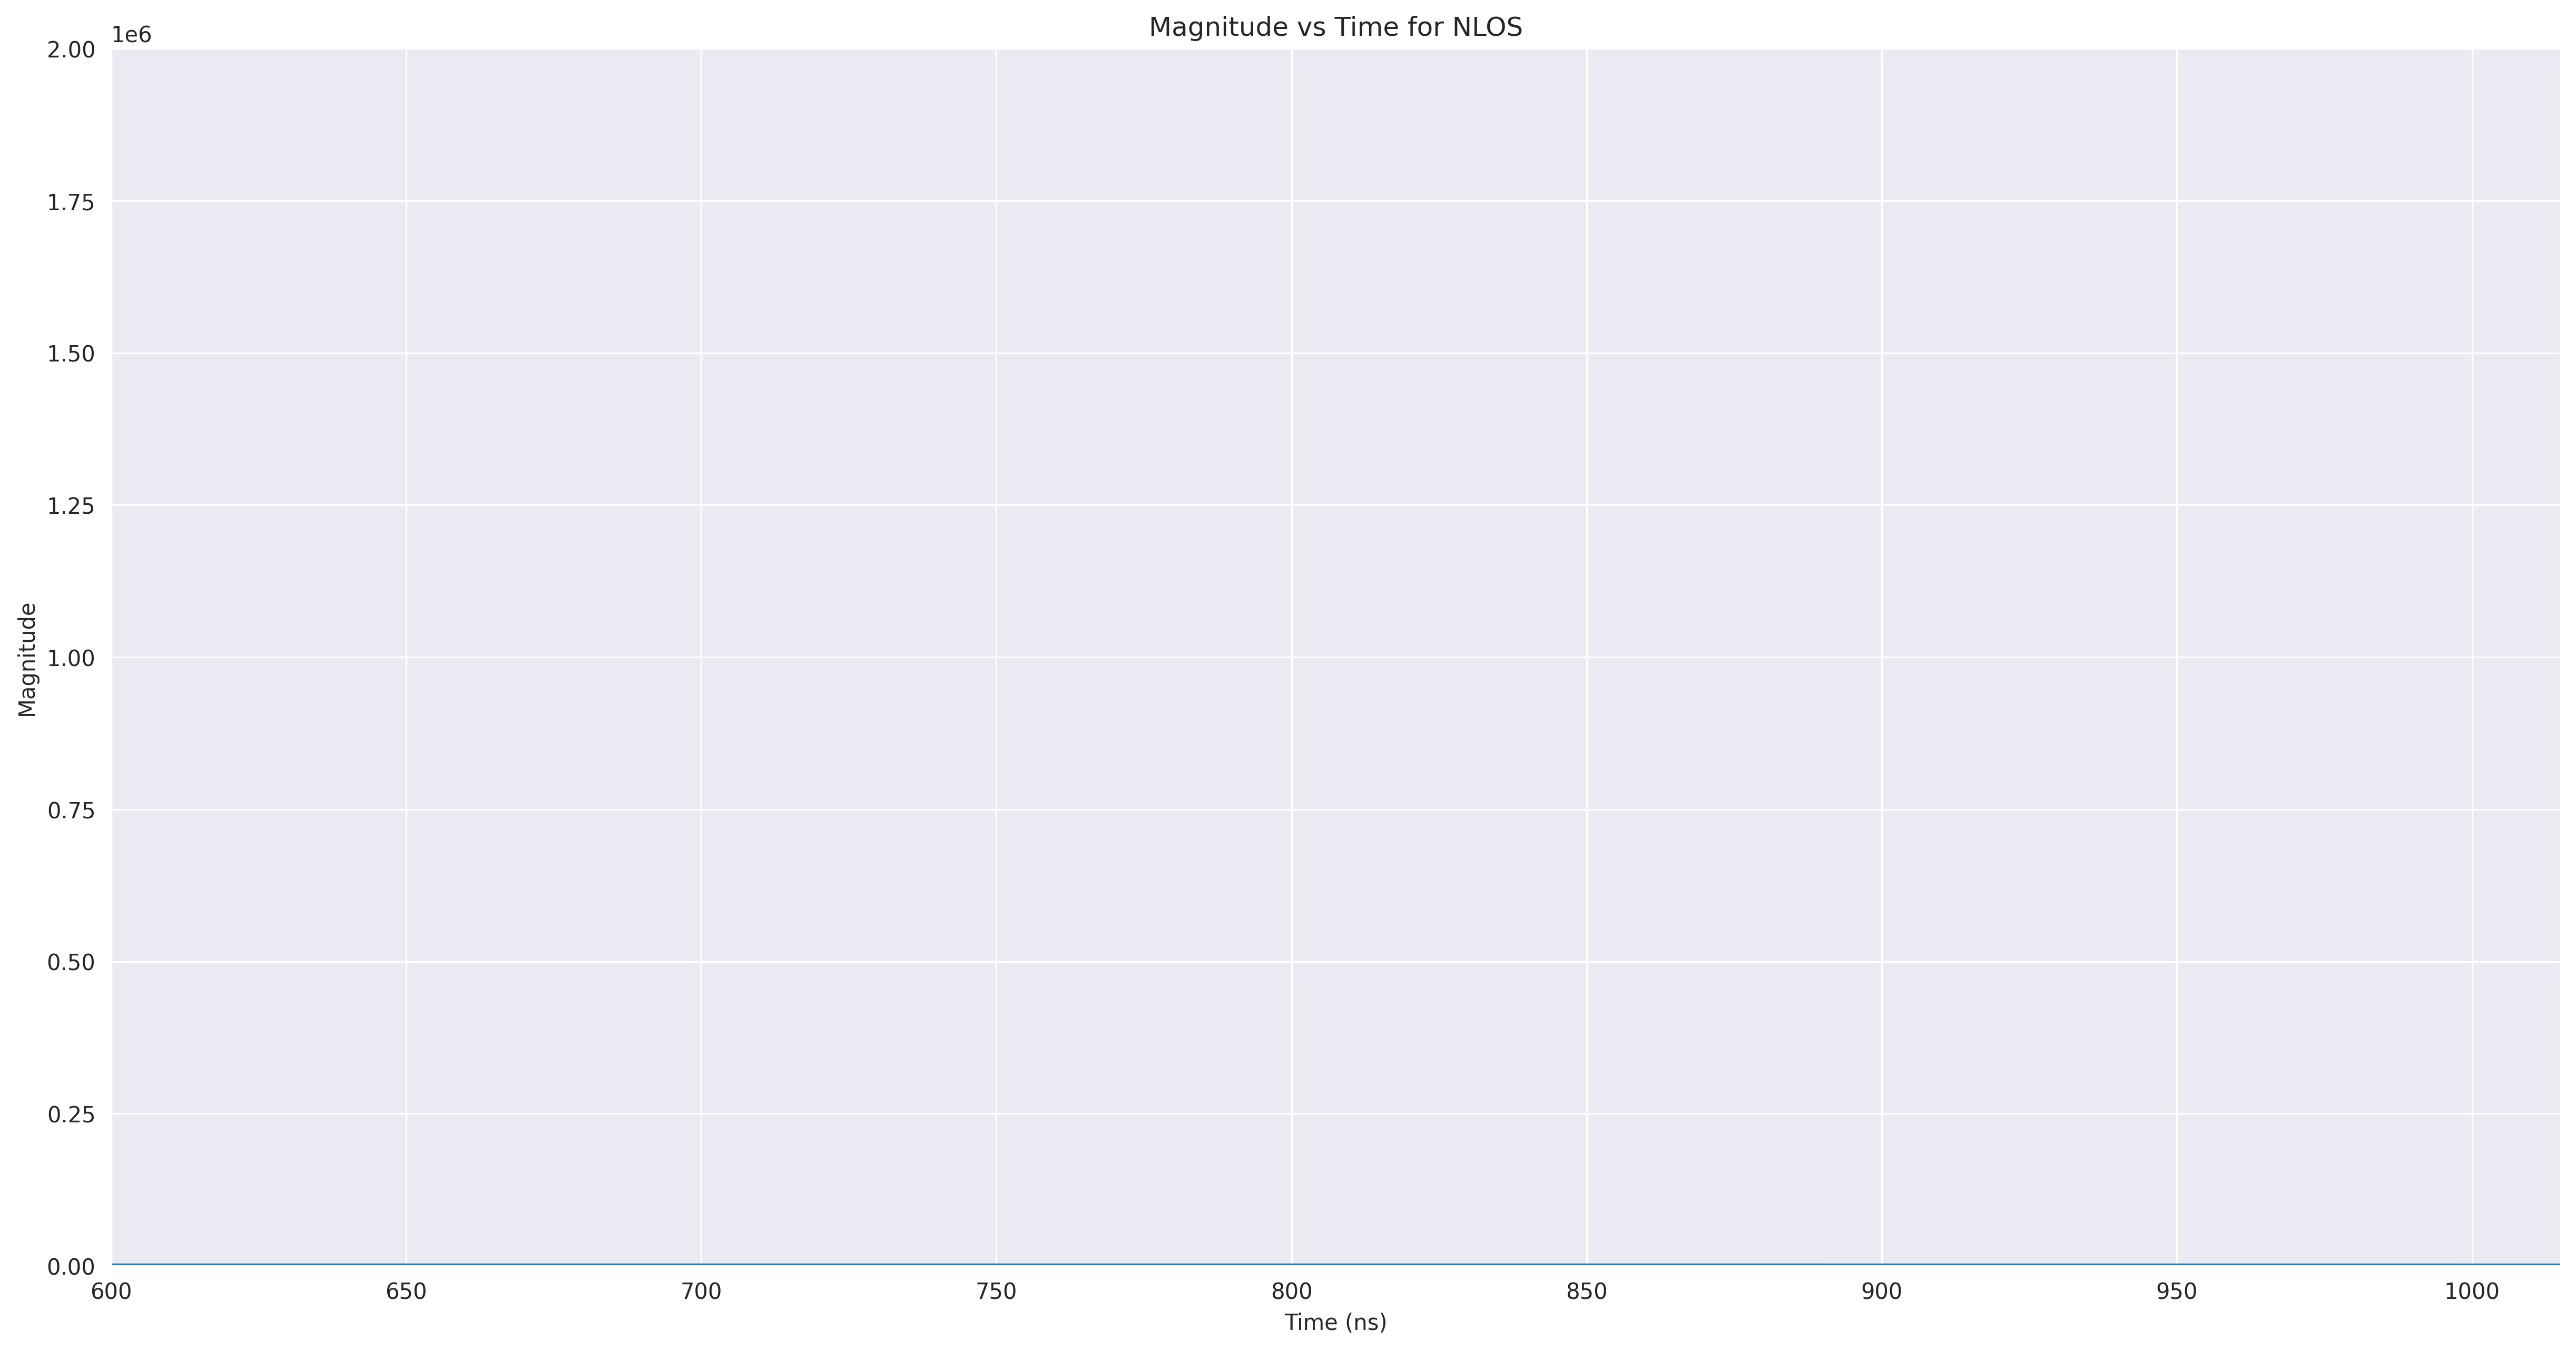
\includegraphics[width=1\textwidth]{preprocessing/lr_denoise_NLOS.png}
  \caption{Frequency Graph of Lucy-Richardson(Unscaled) LOS and NLOS}\label{fig:frequency_graph_lr}
\end{figure}

\begin{figure}[H] 
  \centering
  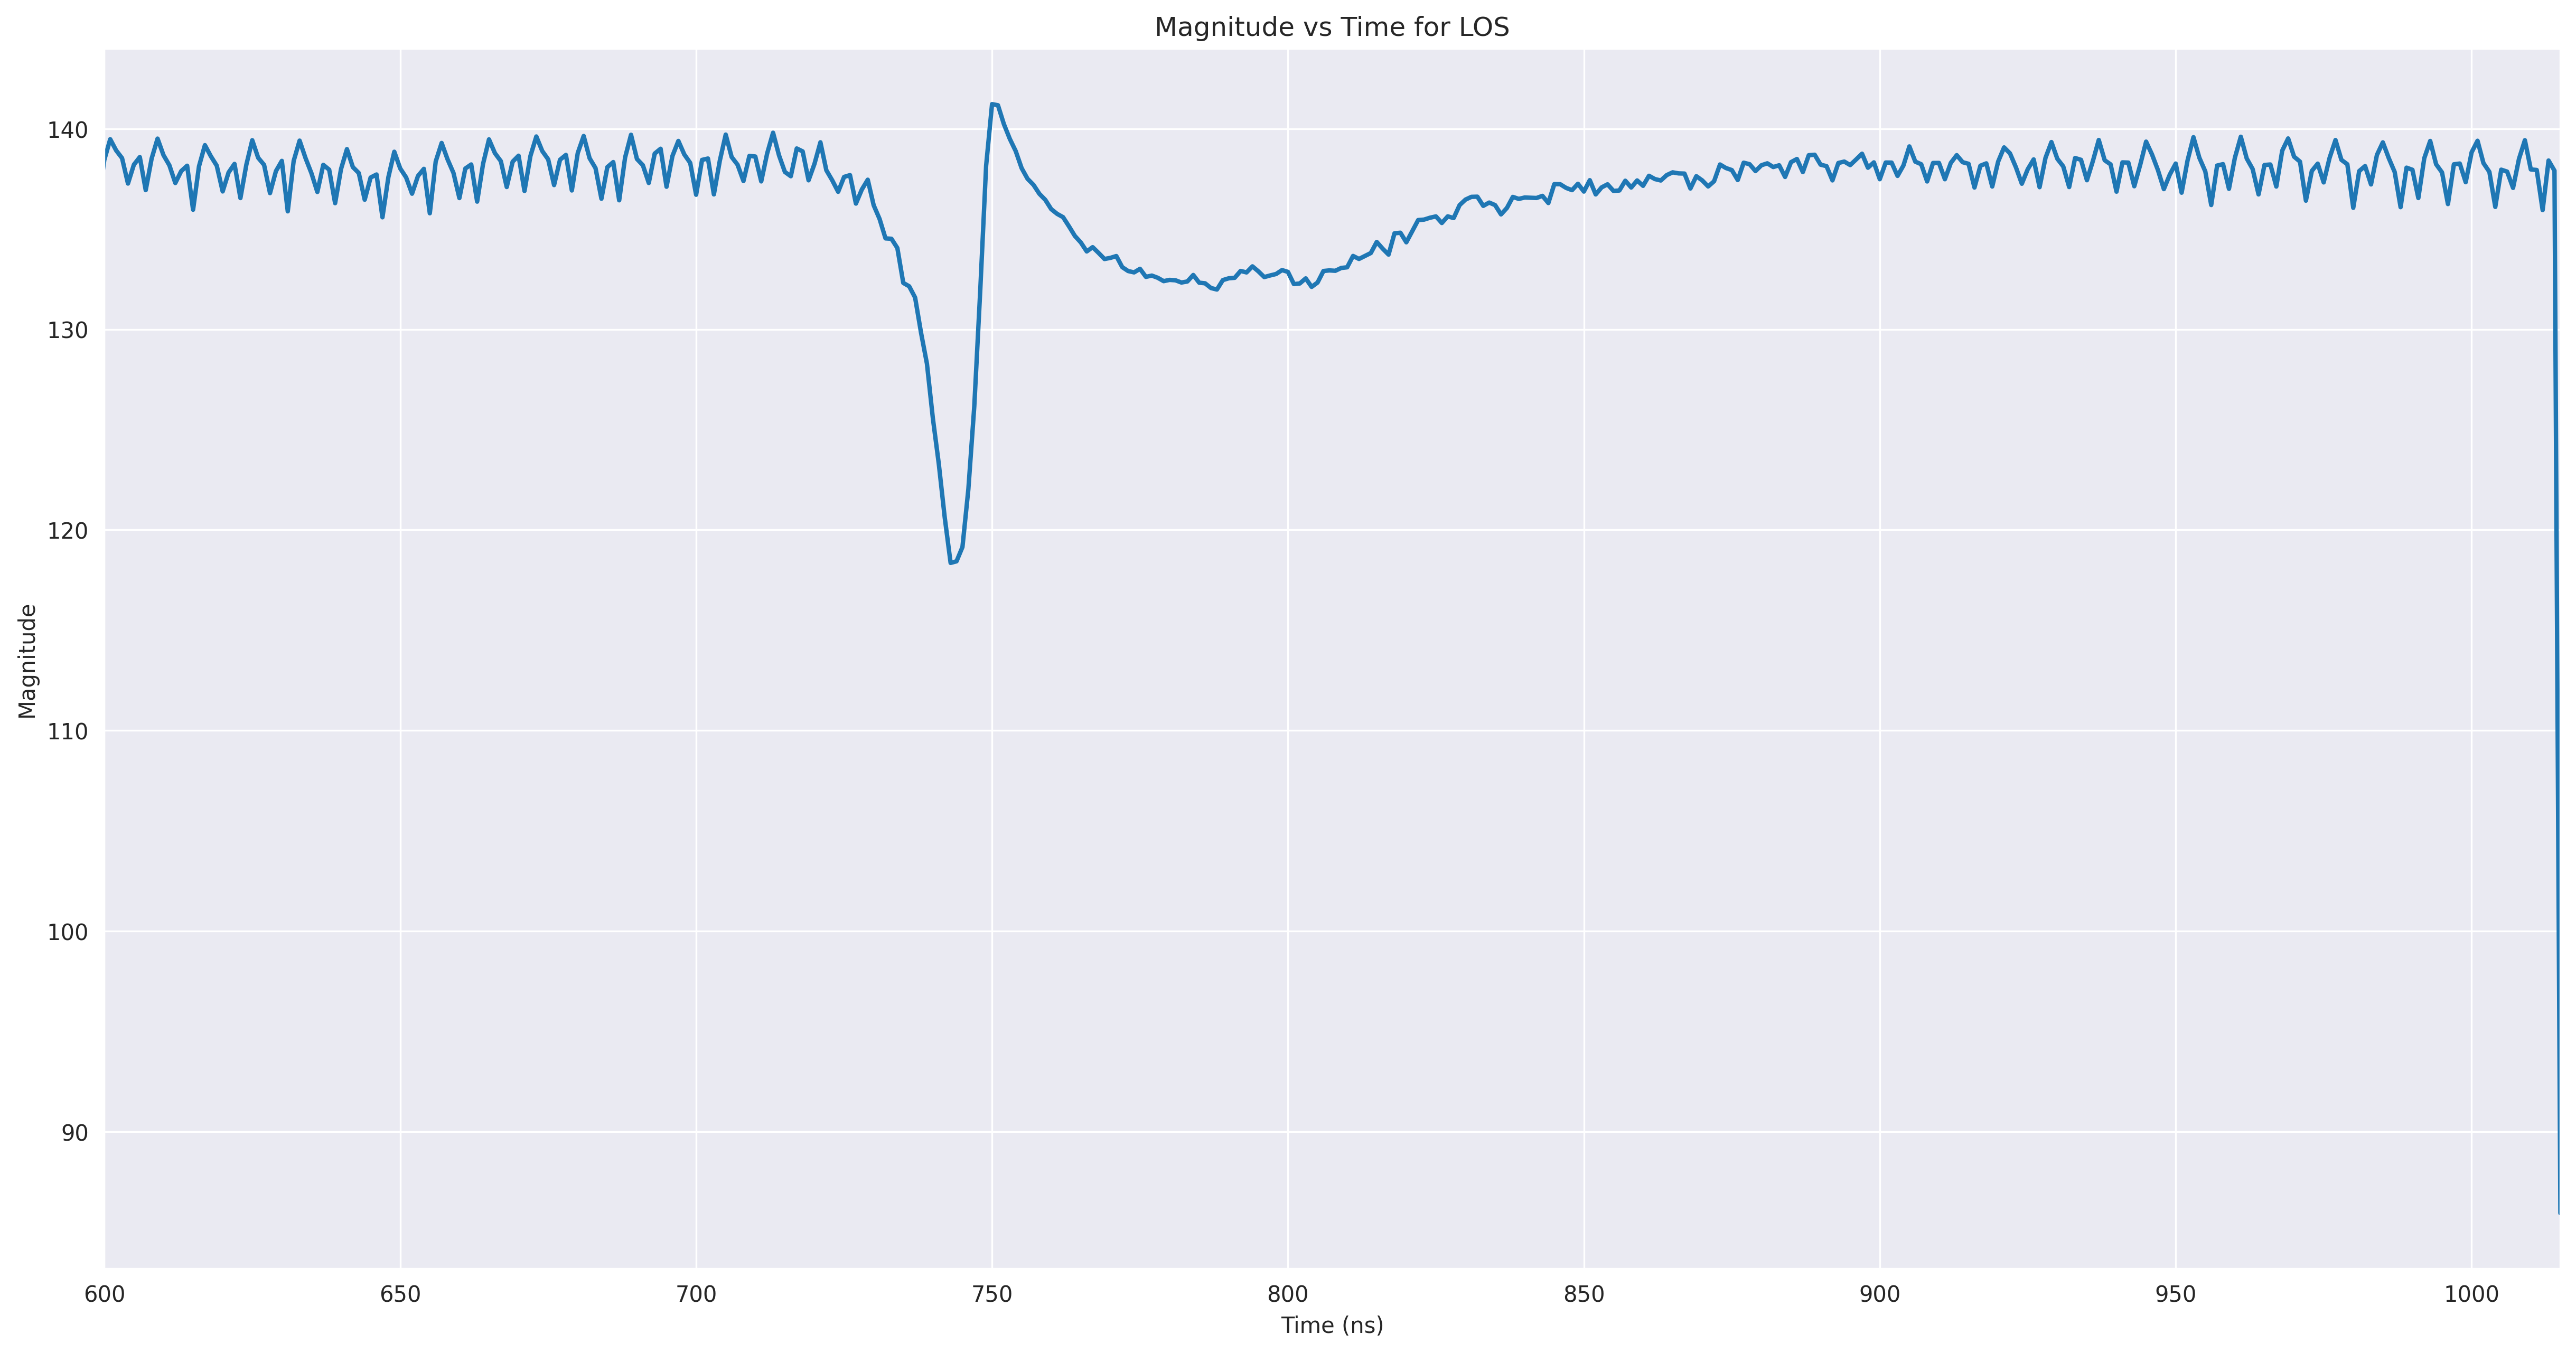
\includegraphics[width=1\textwidth]{preprocessing/lr_denoise_LOS_Scaled.png}
  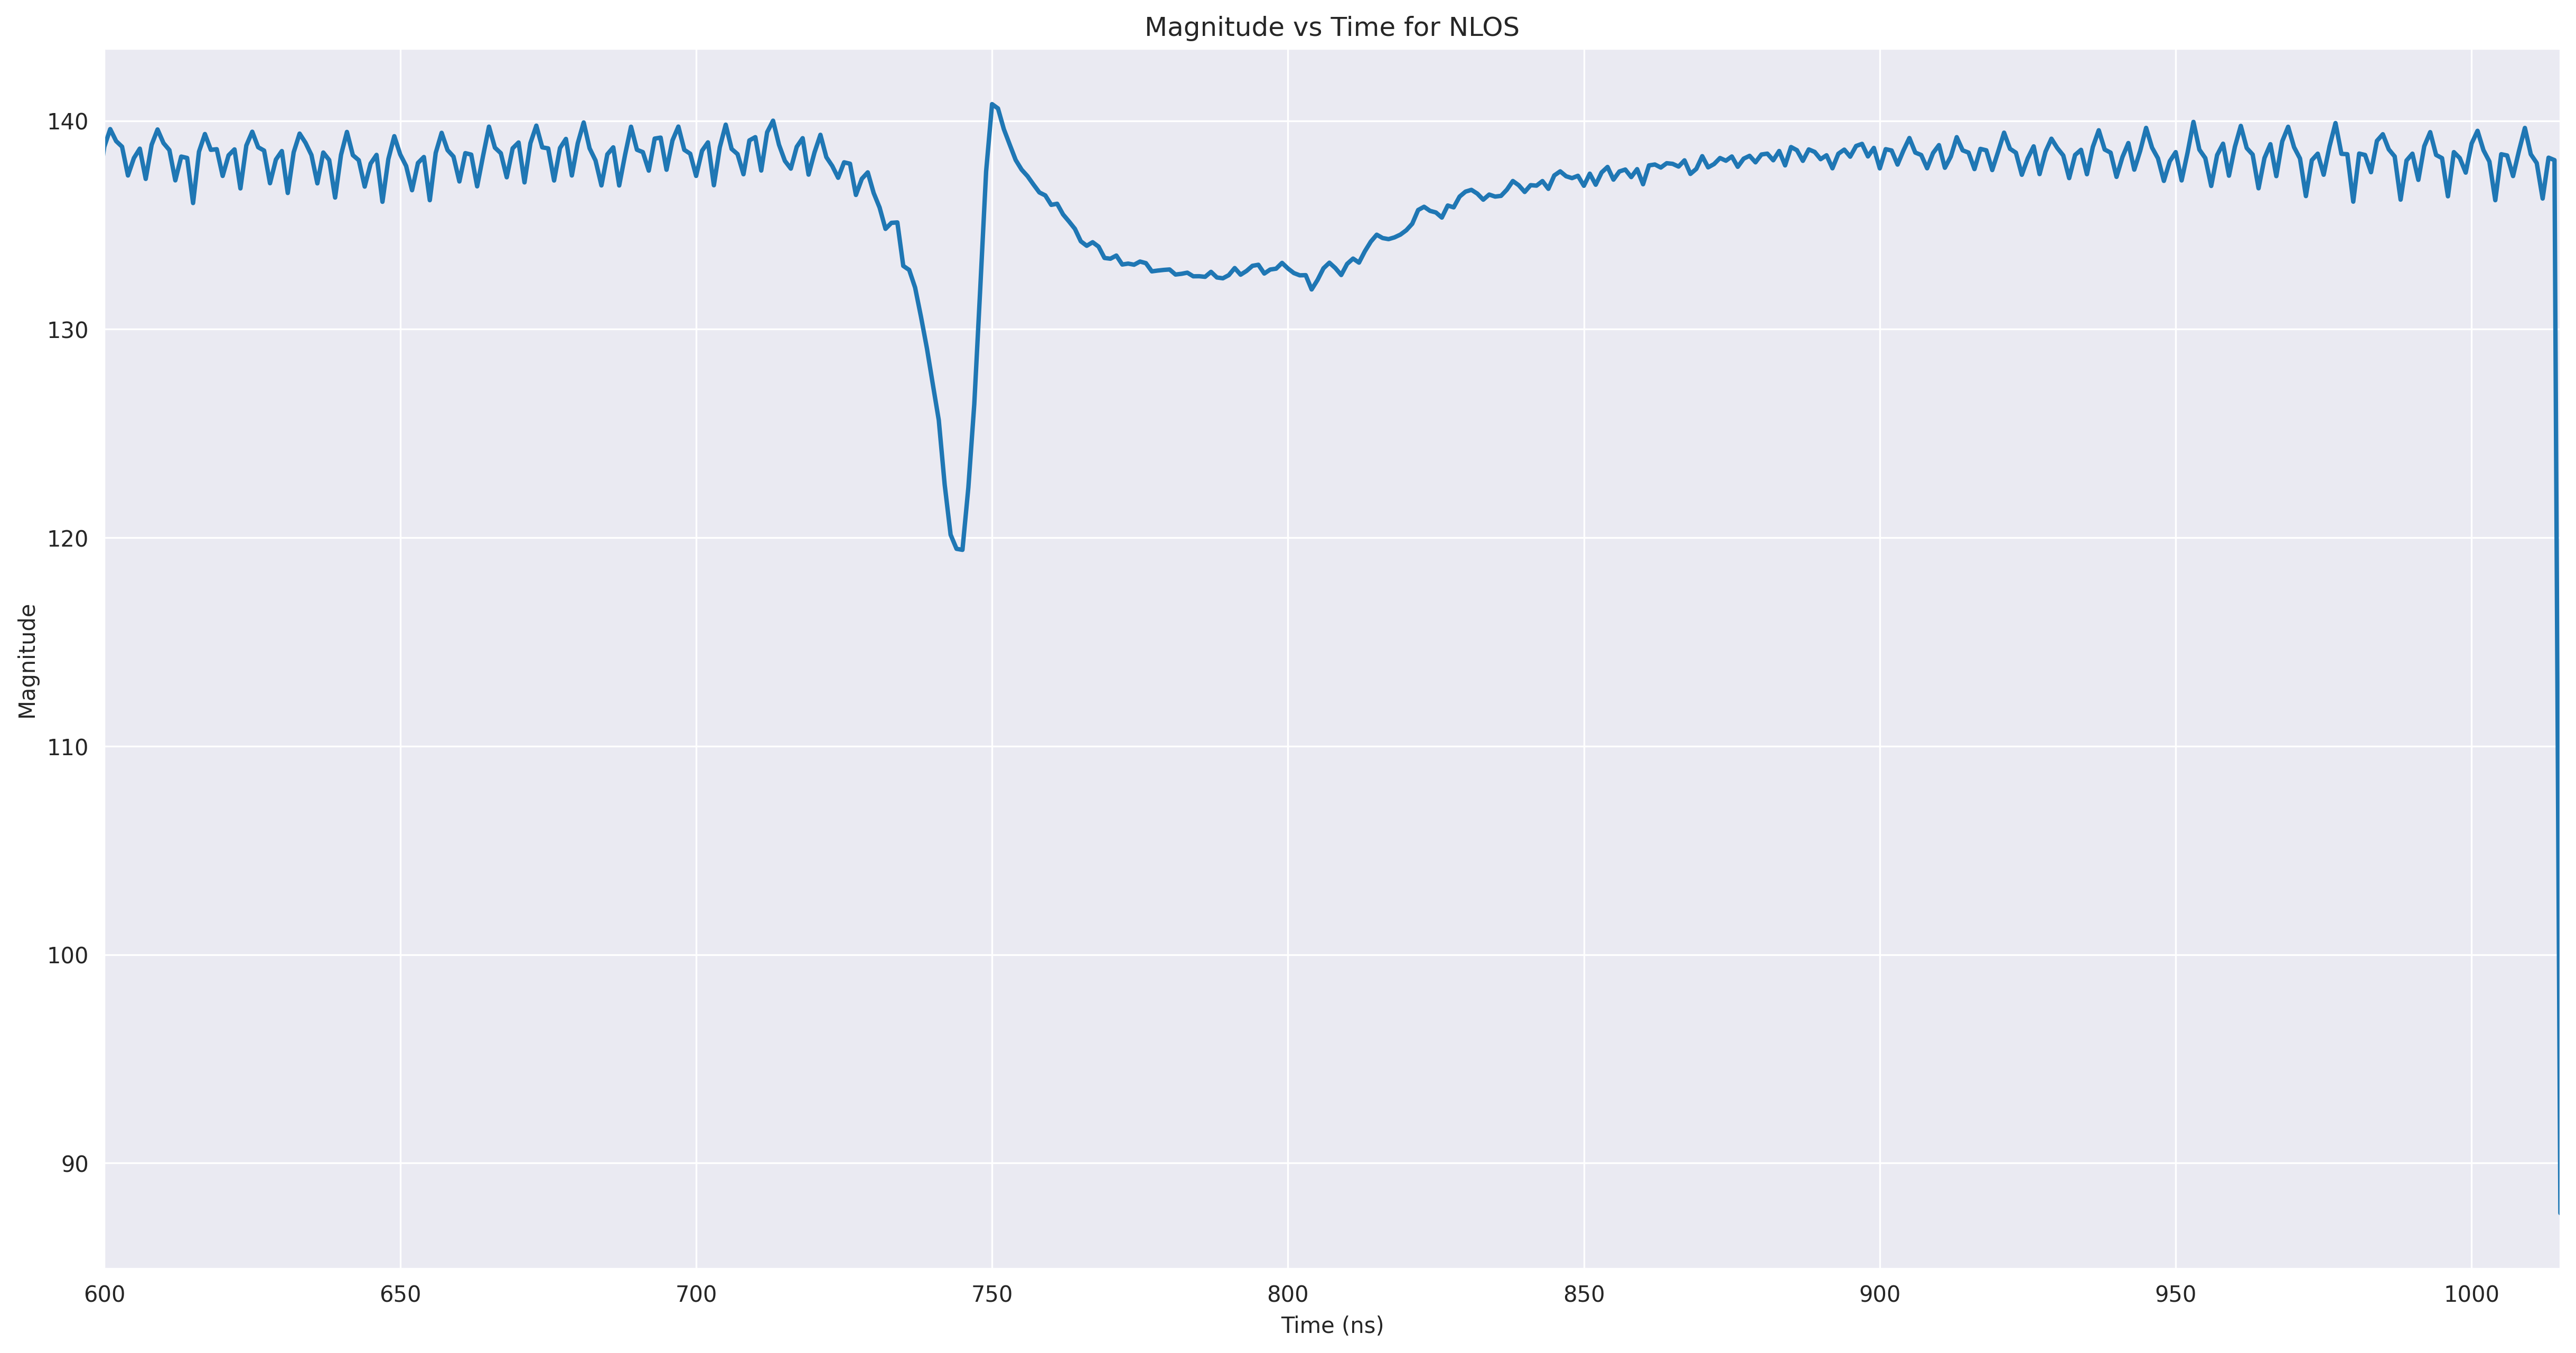
\includegraphics[width=1\textwidth]{preprocessing/lr_denoise_NLOS_Scaled.png}
  \caption{Frequency Graph of Lucy-Richardson(scaled) LOS and NLOS}\label{fig:frequency_graph_lr_scaled}
\end{figure}

\subsubsection{Signal to Noise Ratio}\label{sur_visual}

\begin{figure}[H] % [H] forces the figure to be placed exactly where it appears in the text
	\centering % Horizontally center the figure
	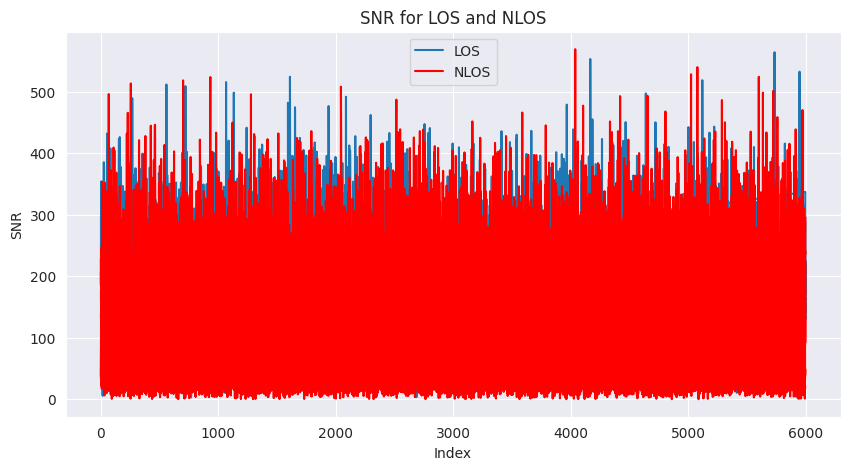
\includegraphics[width=1\textwidth]{preprocessing/SNR} % Include the figure
	\caption{Signal to Noise Ratio}\label{fig:snr}
\end{figure}

%%%%%%%%%%%%%%%%%%%%%%%%%%%%%%%%%%%%%%%%%%%%%%%%%
% CNN Visualisation 
%%%%%%%%%%%%%%%%%%%%%%%%%%%%%%%%%%%%%%%%%%%%%%%%%

\subsection{Convolution Neural Network}\label{cnn_visual}

\begin{figure}[H] 
  \centering
  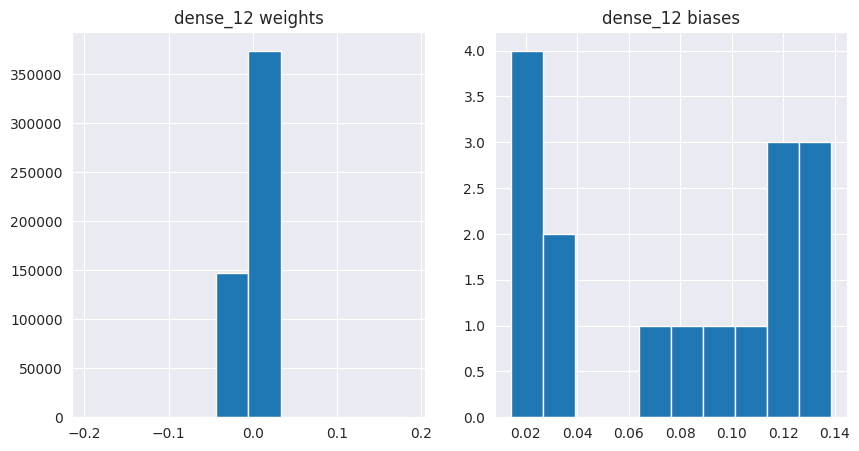
\includegraphics[width=1\textwidth]{cnn/CNN_Weight_Bias1.png}
  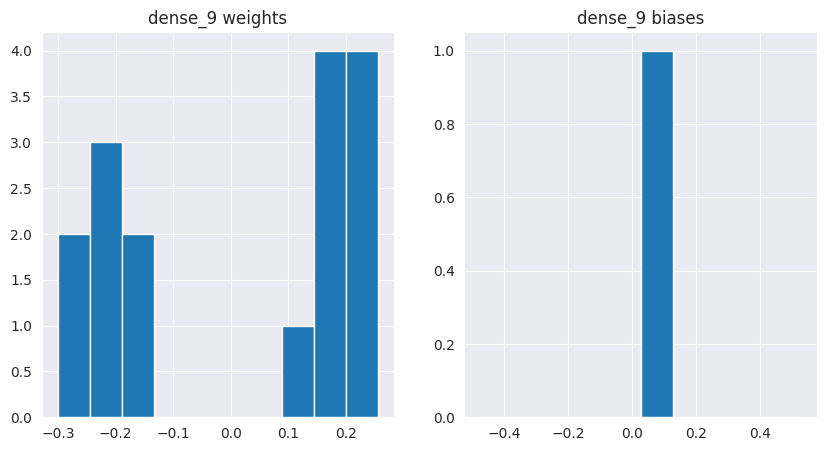
\includegraphics[width=1\textwidth]{cnn/CNN_Weight_Bias2.png}
  \caption{CNN Weights and Biases Evaluation}\label{fig:cnn_weight_bias}
\end{figure}

\begin{figure}[H] 
  \centering
  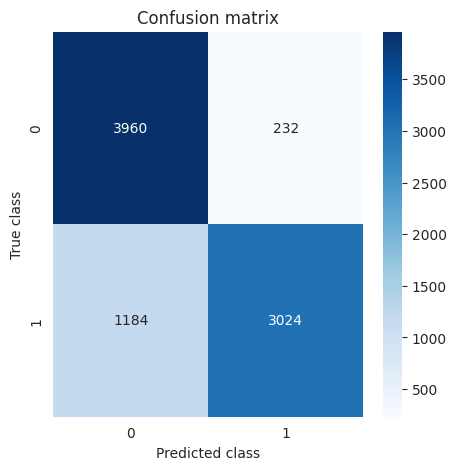
\includegraphics[width=1\textwidth]{cnn/CNN_Confusion_Matrix.png}
  \caption{CNN Confusion Matrix}\label{fig:cnn_confusion_matrix}
\end{figure}

\begin{figure}[H] 
  \centering
  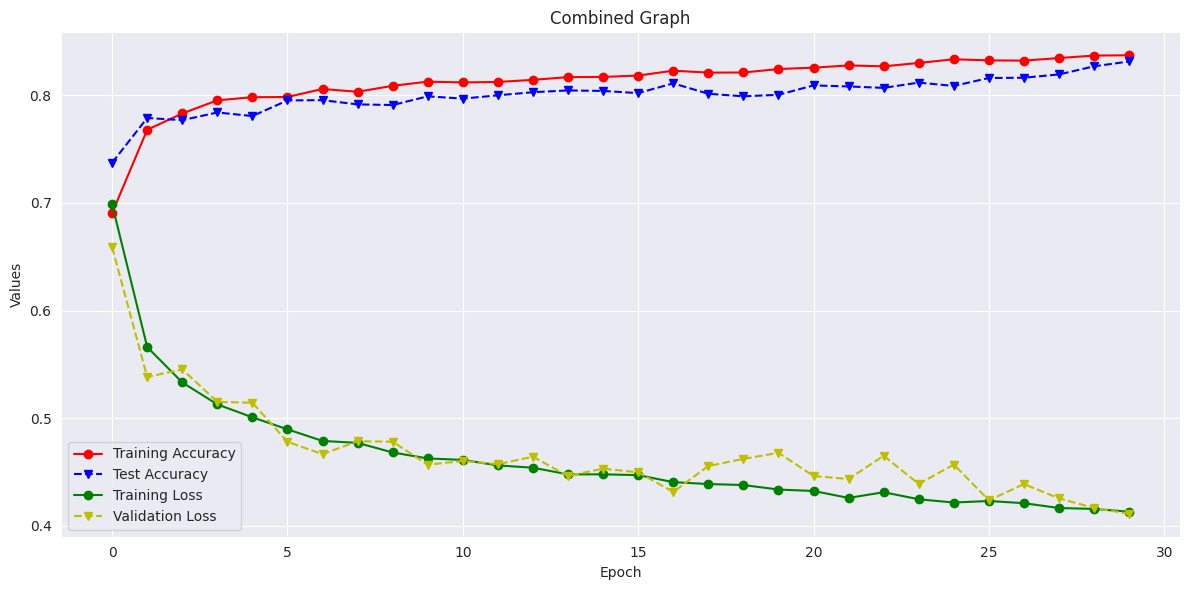
\includegraphics[width=1\textwidth]{cnn/CNN_Learning_Curve.png}
  \caption{CNN Learning Curve}\label{fig:cnn_learning_curve}
\end{figure}

\begin{figure}[H] 
  \centering
  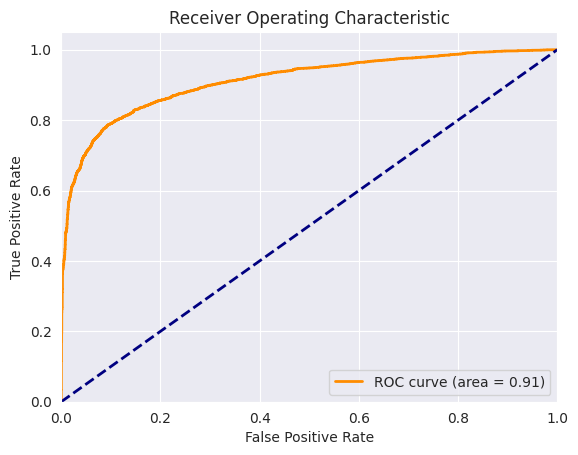
\includegraphics[width=1\textwidth]{cnn/CNN_ROC.png}
  \caption{CNN ROC Curve Evaluation}\label{fig:cnn_roc_curve}
\end{figure}

%%%%%%%%%%%%%%%%%%%%%%%%%%%%%%%%%%%%%%%%%%%%%%%%%
% MLP Visualisation
%%%%%%%%%%%%%%%%%%%%%%%%%%%%%%%%%%%%%%%%%%%%%%%%%

\subsection{Multilayer Perceptron}\label{mlp_visual}

\begin{figure}[H] 
  \centering
  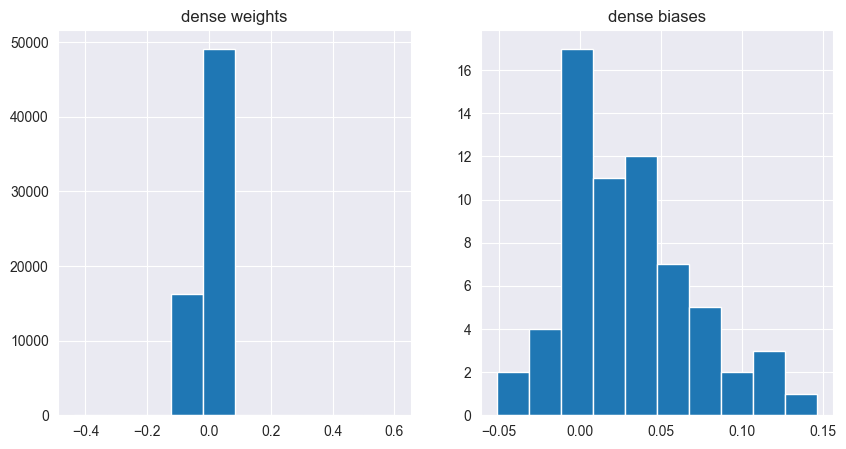
\includegraphics[width=1\textwidth]{mlp/Mlp_dense_biases.png}
  \caption{MLP Weights and Biases Evaluation}\label{fig:mlp_weights_biases}
\end{figure}

\begin{figure}[H] 
  \centering
  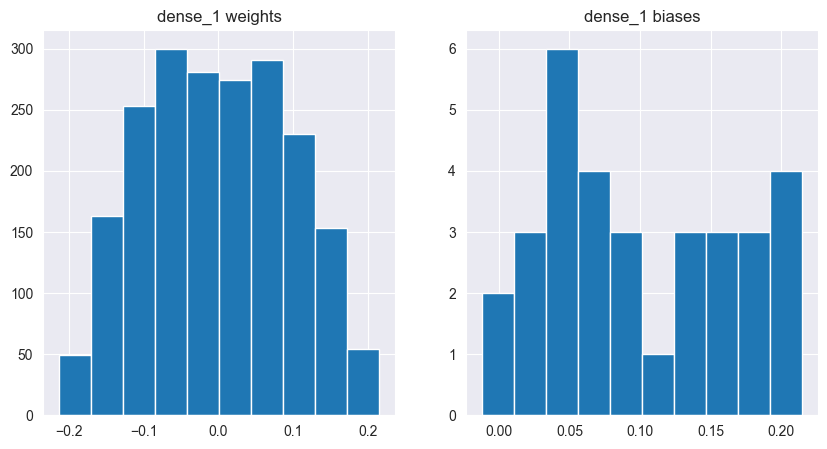
\includegraphics[width=1\textwidth]{mlp/Mlp_dense1_bias1.png}
  \caption{MLP Weights and Biases Evaluation}\label{fig:dense1_bias1}
\end{figure}

\begin{figure}[H] 
  \centering
  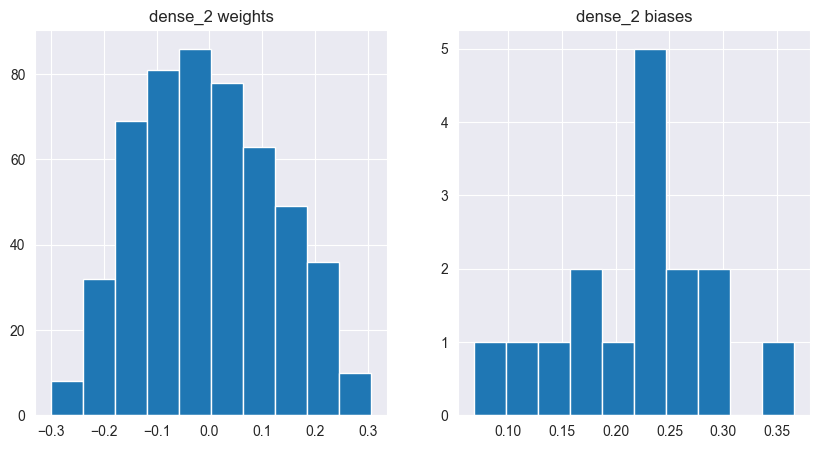
\includegraphics[width=1\textwidth]{mlp/Mlp_dense2_bias2.png}
  \caption{MLP Weights and Biases Evaluation}\label{fig:dense2_bias2}
\end{figure}

\begin{figure}[H] 
  \centering
  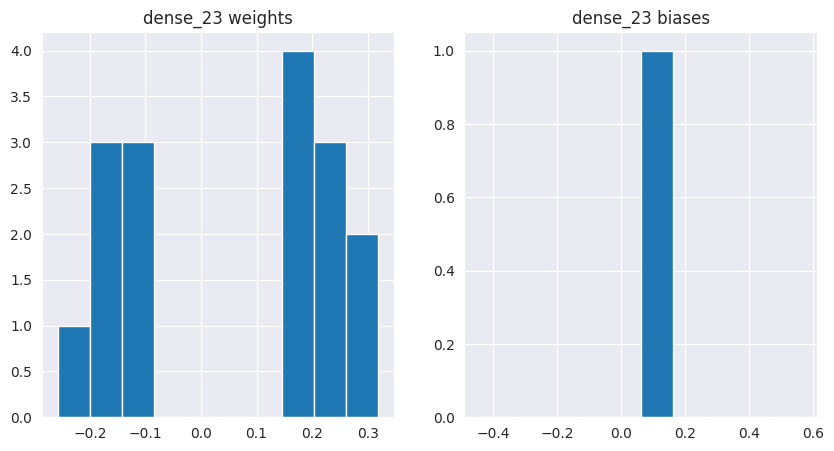
\includegraphics[width=1\textwidth]{mlp/Mlp_dense3_bias3.png}
  \caption{MLP Weights and Biases Evaluation}\label{fig:dense3_bias3}
\end{figure}

The weights and biases of the MLP model layers were visualized to understand their distributions. The weights in all layers (dense_20, dense_21, dense_22, and dense_23) are not close to zero, indicating they are likely being updated during training and contributing to the model’s learning. The weight distributions show a spread around zero, suggesting the model is capturing complex relationships in the data.

The biases in dense_20 and dense_22 introduce a slight positive bias to the activations in subsequent layers, potentially affecting the model’s predictions. The biases in dense_21 and dense_23 are centered around zero, with a slight spread towards positive values, introducing a small positive shift in the activations of the next layer.

The impact of these biases would depend on the network architecture and data. Overall, the model’s weights and biases suggest that it is learning effectively from the training data.

\begin{figure}[H] 
  \centering
  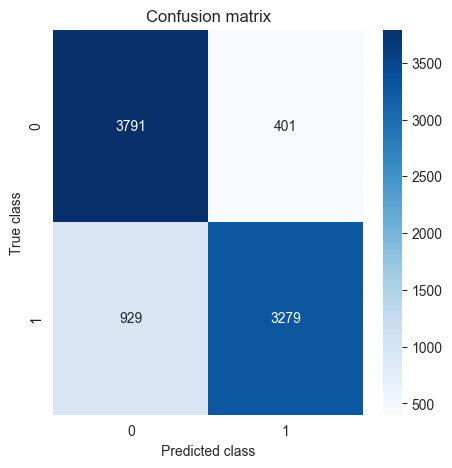
\includegraphics[width=1\textwidth]{mlp/Mlp_confusion_matrix.png}
  \caption{MLP Confusion Matrix}\label{fig:mpl_confusion_matrix}
\end{figure}

the MLP model performs admirably in categorizing NLOS/LOS signals, accurately identifying 3791 LOS signals (True Positives) and 3279 NLOS signals (True Negatives). However, it erroneously categorizes 401 NLOS signals as LOS (False Positives) and 929 LOS signals as NLOS (False Negatives). Although the model achieves a high overall accuracy by correctly classifying a considerable number of samples, the asymmetry in errors, particularly the higher number of False Negatives for LOS signals, suggests areas for improvement. This discrepancy may stem from the broader range of variations present in LOS signals compared to NLOS signals, indicating the need for further refinement to enhance the model's accuracy and balance in classification.

\begin{figure}[H] 
  \centering
  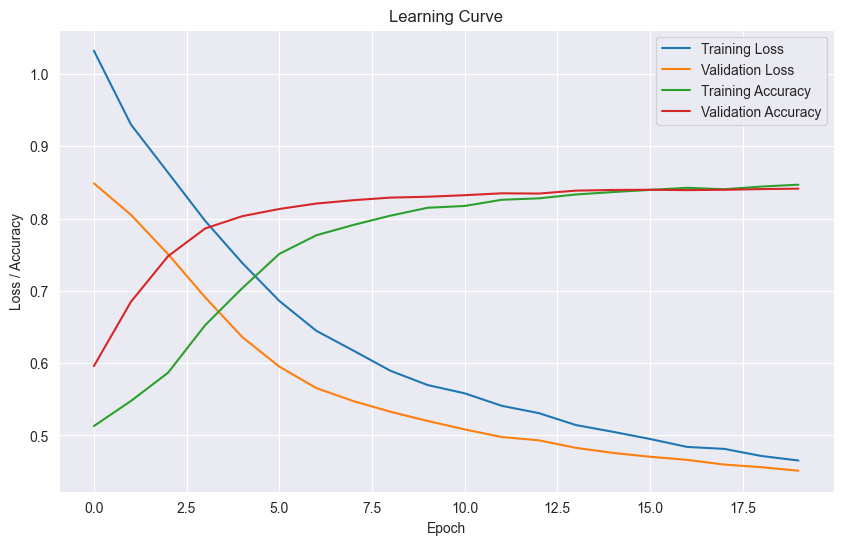
\includegraphics[width=1\textwidth]{mlp/Mlp_learning_curve.png}
  \caption{MLP Learning Curve}\label{fig:mlp_learning_curve}
\end{figure}

Positive indicators observed from the mlp learning curve includes the steadily increasing training accuracy, indicating the model is effectively learning patterns in the NLOS/LOS signal data over the 20 epochs. The rising validation accuracy suggests the model is successfully generalizing these learned patterns to new, unseen data, thereby avoiding overfitting. Additionally, the relatively small gap between the training and validation curves further supports the notion of good generalization and minimal overfitting. However, there is potential for further improvement, as the validation curves show signs of plateauing around epoch 20, indicating the model may be nearing its optimal performance on the validation data.

\begin{figure}[H] 
  \centering
  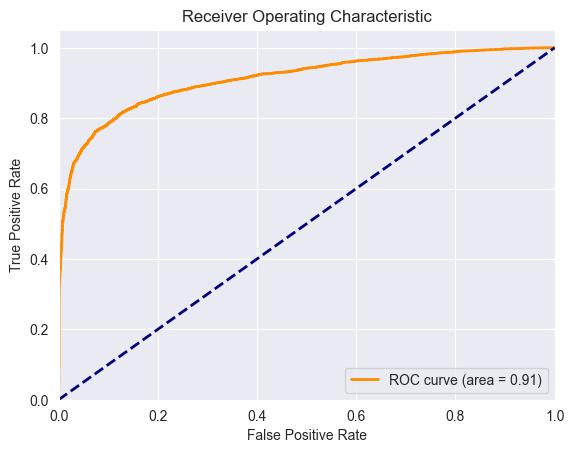
\includegraphics[width=1\textwidth]{mlp/Mlp_ROC_Curve.png}
  \caption{MLP ROC Curve Evaluation}\label{fig:mpl_roc_curve}
\end{figure}

The area under the ROC curve (AUC) is approximately 0.91, indicating strong model performance. The ROC curve illustrates the True Positive Rate (TPR) against the False Positive Rate (FPR) at different classification thresholds. The AUC signifies the probability of the model ranking a randomly selected positive instance (LOS) higher than a randomly selected negative instance (NLOS) across all thresholds, with 1 indicating perfect performance and 0.5 indicating chance performance.

The model's AUC of 0.91 suggests that the MLP model effectively distinguishes between NLOS and LOS signals, with a high likelihood of ranking true LOS signals higher than non-LOS signals and overall, this means that the MLP model is a strong classifier for NLOS/LOS signals.
